\documentclass[aspectratio=169]{beamer}
\usepackage{CustomTheme}

\usepackage{colortbl} 
\usepackage{diagbox}
\usepackage{tikz}
\usepackage{tikz-qtree}
\usepackage{csquotes}


\title[NLP 4 CH]{Lemmatization }
\date[2024] % (optional)
{Natural Language Processing for CH}
\addbibresource{nlp-for-ch/03-Lemmatization.bib}


\begin{document}

\frame{
\maketitle
}

\section{Lemmatization and "Grammatical" tasks}

% Definition of lemmatization and related tasks
% Different lemmatization models and the different errors that can occur

\begin{frame}{What is Lemmatization?}

\begin{quote}
``In computational linguistics, lemmatization is the algorithmic process of determining the lemma of a word based on its intended meaning. Unlike stemming, lemmatization depends on correctly identifying the intended part of speech and meaning of a word in a sentence, as well as within the larger context surrounding that sentence, such as neighbouring sentences or even an entire document. As a result, developing efficient lemmatization algorithms is an open area of research.''
\end{quote}
\signed{Lemmatization, Wikipedia (October 18, 2024)}
\end{frame}

\begin{frame}{Example of Lemmatization}
\begin{center}%
\begin{tabular}{l|llllllll}
\textit{Texte}         & Les & étoiles & luisent & dans & la & nuit & noire & . \\ \hline
\textit{Lemmatisation} & le  & étoile  & luire   & dans & le & nuit & noir  & .
\end{tabular}
\end{center}

\pause

\textbf{2 forms out of 8} (25\%) can only be lemmatized in one way, regardless of the context (in modern French): punctuation (\texttt{.}) and the preposition (\texttt{est}).

\pause
\vspace{1em}

In lemmatization, many lemmas are \textit{easy} to choose (punctuation and invariable words: only one lemma choice). On the other end of the spectrum, for machines, are homographs or irregular forms: “est” for “être” does not follow the common structure of other verbs and is also a homograph: “elle est allée vers l'est.” To choose the lemma, the context of the lexeme is necessary.
\end{frame}

\begin{frame}{Other Tasks: POS}

\begin{itemize}
    \item \textbf{POS}: \textit{Part-of-speech}
    \item Translatable as "part of speech" in traditional grammar
    \item More precisely: a set of grammatical (not semantic) categorizations based on syntactic distributions, syntactic functions, and acceptable morphologies.
    \item Importance of the information: \begin{itemize}
        \item Automatic analyses (stylometry, general text classification)
        \item Category-based search (Search for all proper nouns, all adjectives, etc.)
    \end{itemize}
\end{itemize}
    
\end{frame}

\begin{frame}{Other Tasks: Morphological Annotation}

\begin{itemize}
    \item Set of morphological information (mood, tense, number, gender, etc.)
    \item In some cases, projects have chosen not to disambiguate. Morphology is not "that" simple: “the boys and girls left”; two possibilities, masculine plural or create a masculine+feminine plural category.
    \item Importance of the information: \begin{itemize}
        \item Automatic analyses (stylometry, general text classification)
        \item Category-based search (Search for all feminine adjectives and masculine ones, study their distribution, etc.)
        \item Linguistic study of a text as part of an edition.
    \end{itemize}
\end{itemize}
    
\end{frame}

\begin{frame}{Other Tasks: NER}

\begin{itemize}
    \item \textbf{NER(D)}: Named Entity Recognition (and Disambiguation)
    \item Recognizing that lexemes or groups of lexemes represent places, organizations, and people in a corpus.
    \item Importance of the information: \begin{itemize}
        \item Automatic analyses (stylometry, general text classification)
        \item Category-based search (what are the places in tragic texts?)
        \item Index creation
    \end{itemize}
\end{itemize}
    
\end{frame}

\section{Tools and their structure}

\begin{frame}{Collatinus}
    \centering
    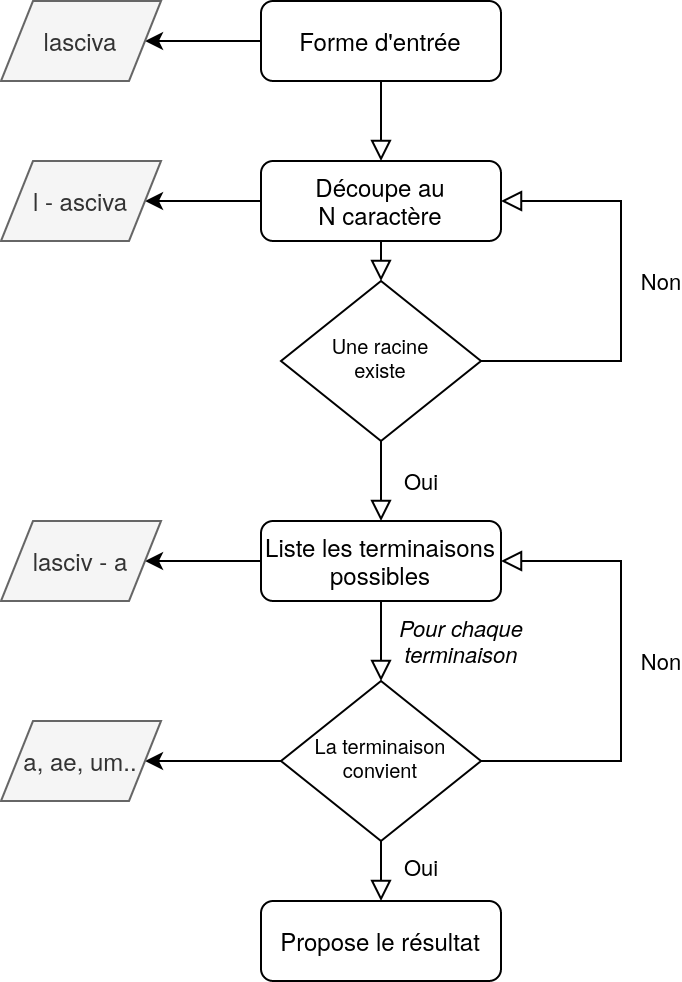
\includegraphics[height=\textheight]{nlp-for-ch/images/collatinus.png}
\end{frame}

\begin{frame}{Machine Learning and Statistics}
    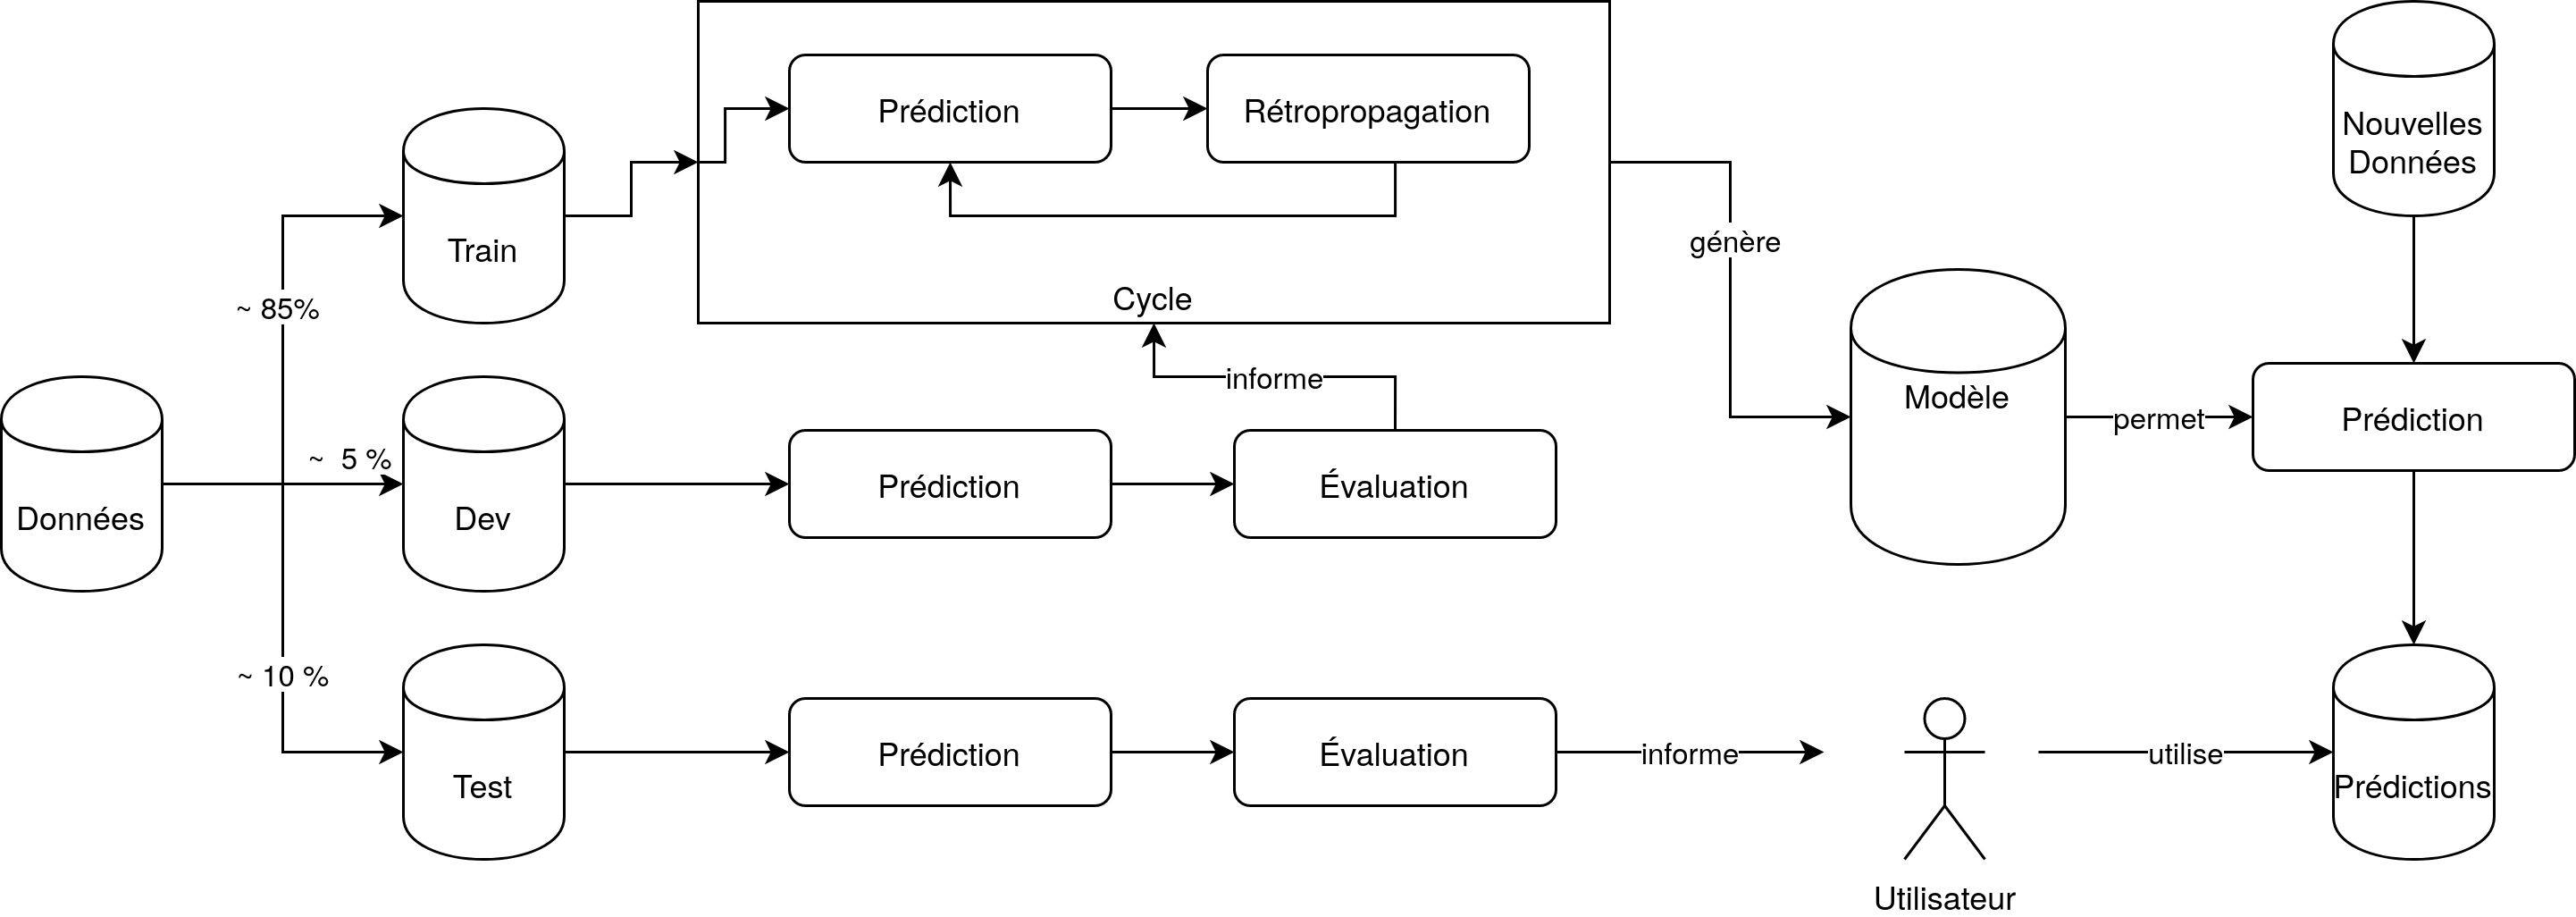
\includegraphics[width=\textwidth]{nlp-for-ch/images/MachineLearning.png}
\end{frame}

\begin{frame}{TreeTagger}
    \centering
    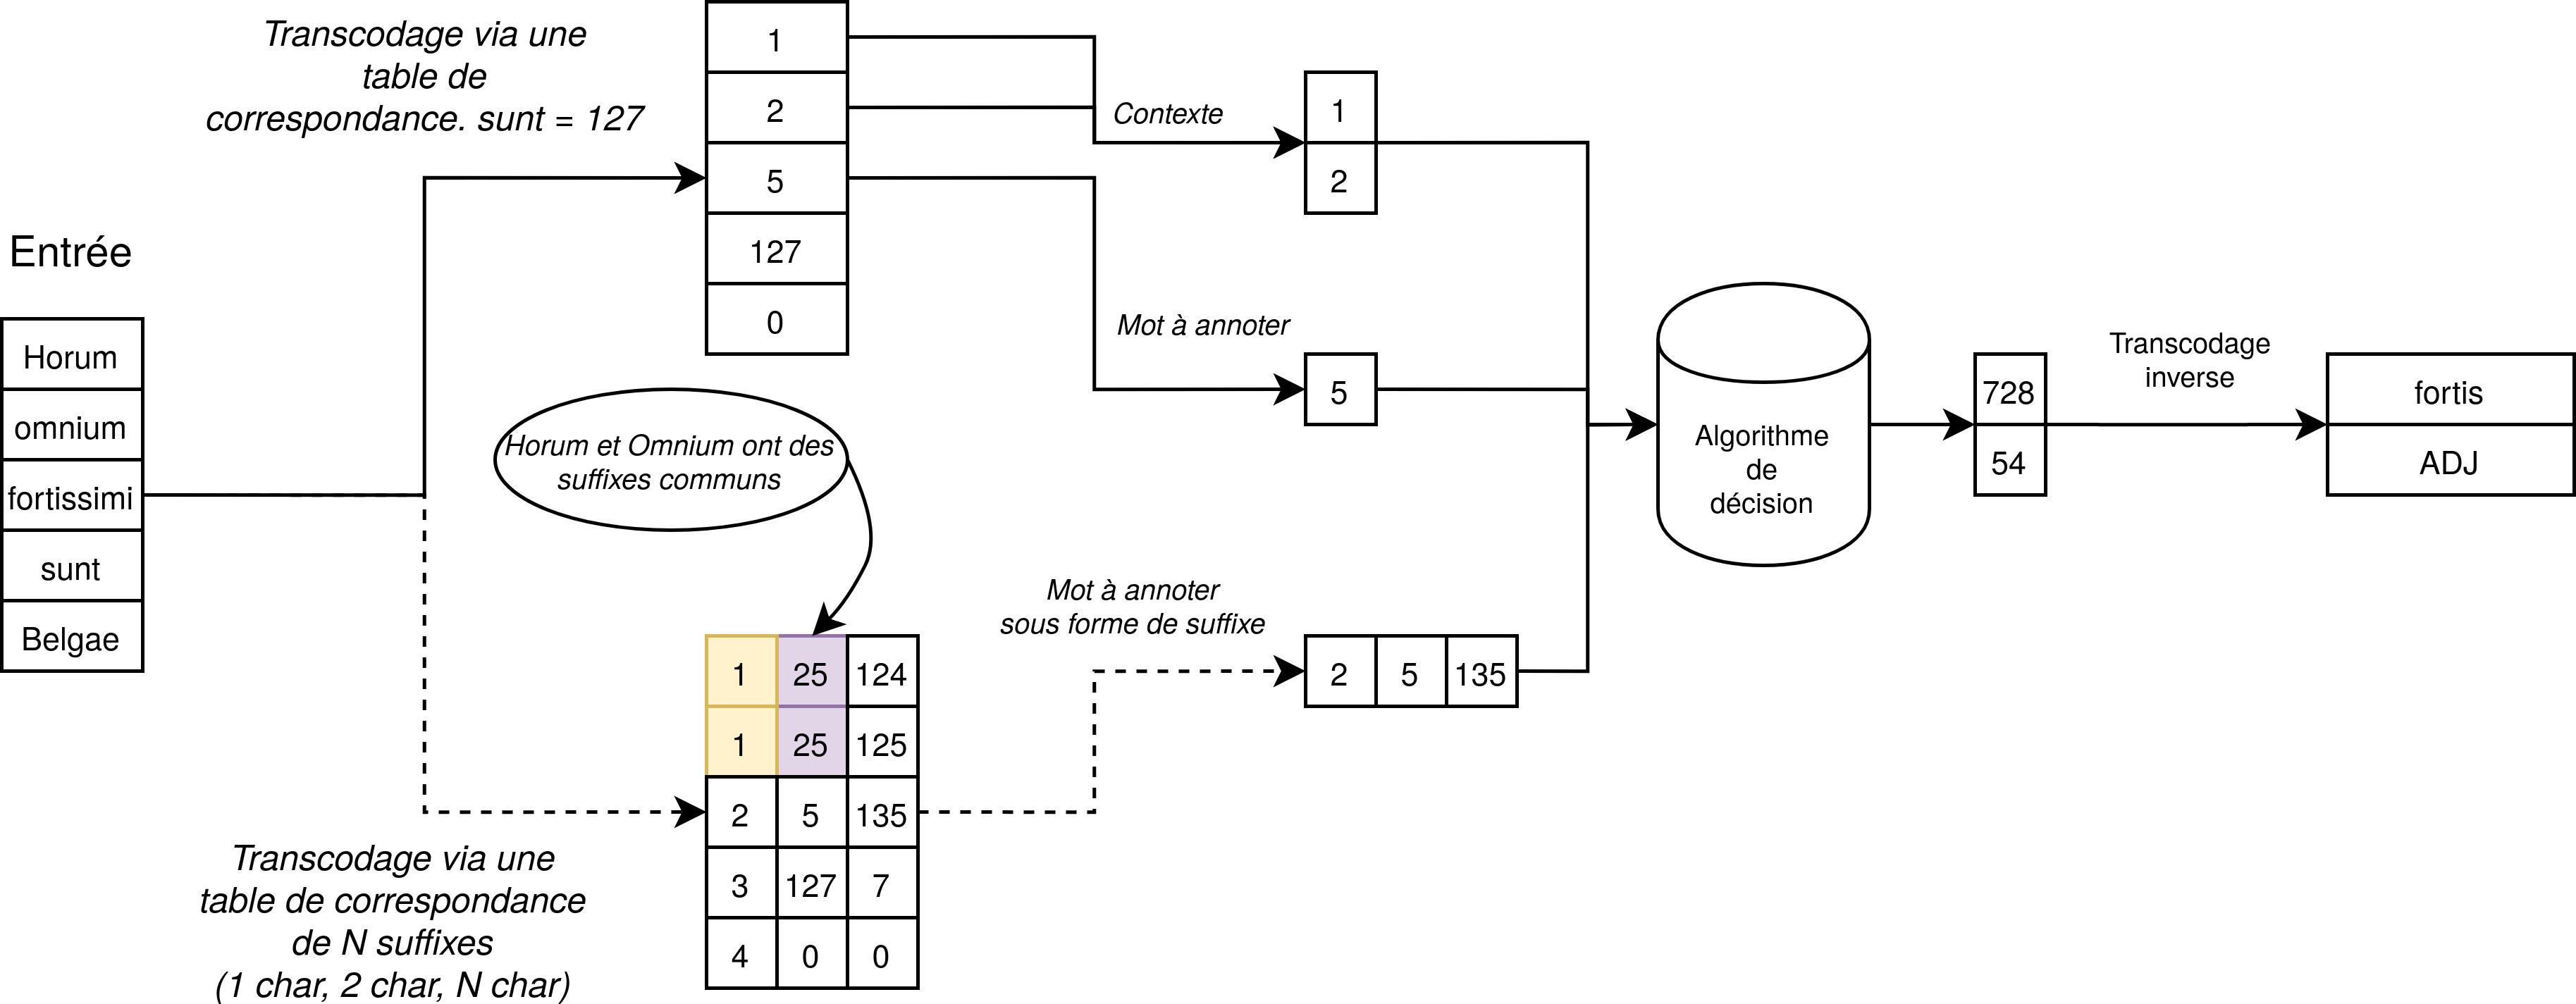
\includegraphics[width=\textwidth]{nlp-for-ch/images/treetagger_type.png}
\end{frame}

\begin{frame}{Plank et al., 2016}
    \begin{columns}
        \begin{column}{.5\textwidth}
            \fullcite{plank-etal-2016-multilingual}
        \end{column}
        \begin{column}{.5\textwidth}
            \centering
            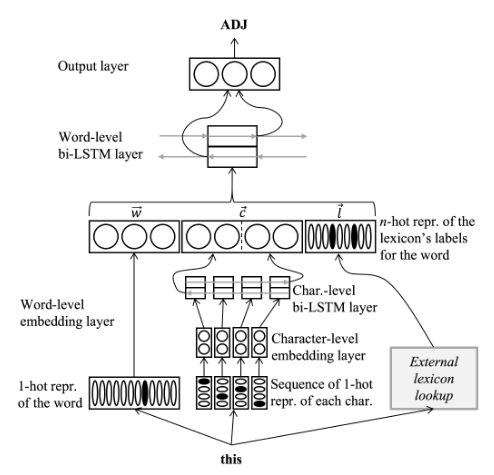
\includegraphics[height=.8\textheight]{nlp-for-ch/images/planketal.png}
        \end{column}
    \end{columns}
\end{frame}

\begin{frame}{Sagot et Alonso, 2017}
    \begin{columns}
        \begin{column}{.5\textwidth}
            \fullcite{sagot-martinez-alonso-2017-improving}
        \end{column}
        \begin{column}{.5\textwidth}
            \centering
            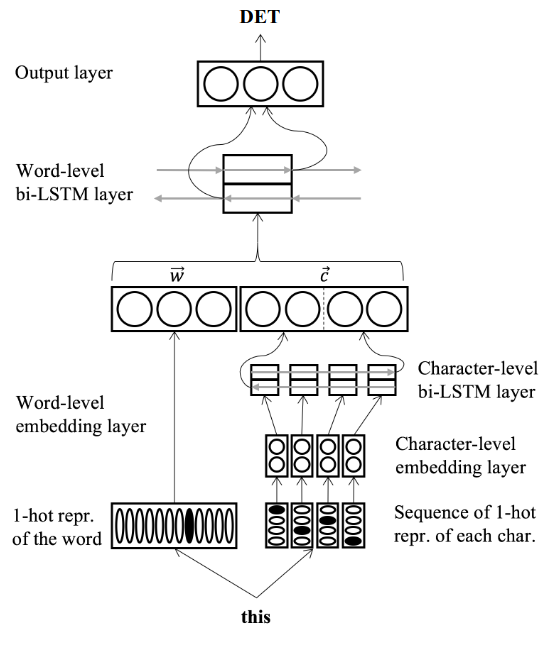
\includegraphics[height=.8\textheight]{nlp-for-ch/images/Plank.png}
        \end{column}
    \end{columns}
\end{frame}


\begin{frame}{Manjavacas et al., 2019 -- Pie}
    \vspace{1.5em}
    {\tiny \fullcite{manjavacas-etal-2019-improving}}
    
    \centering
    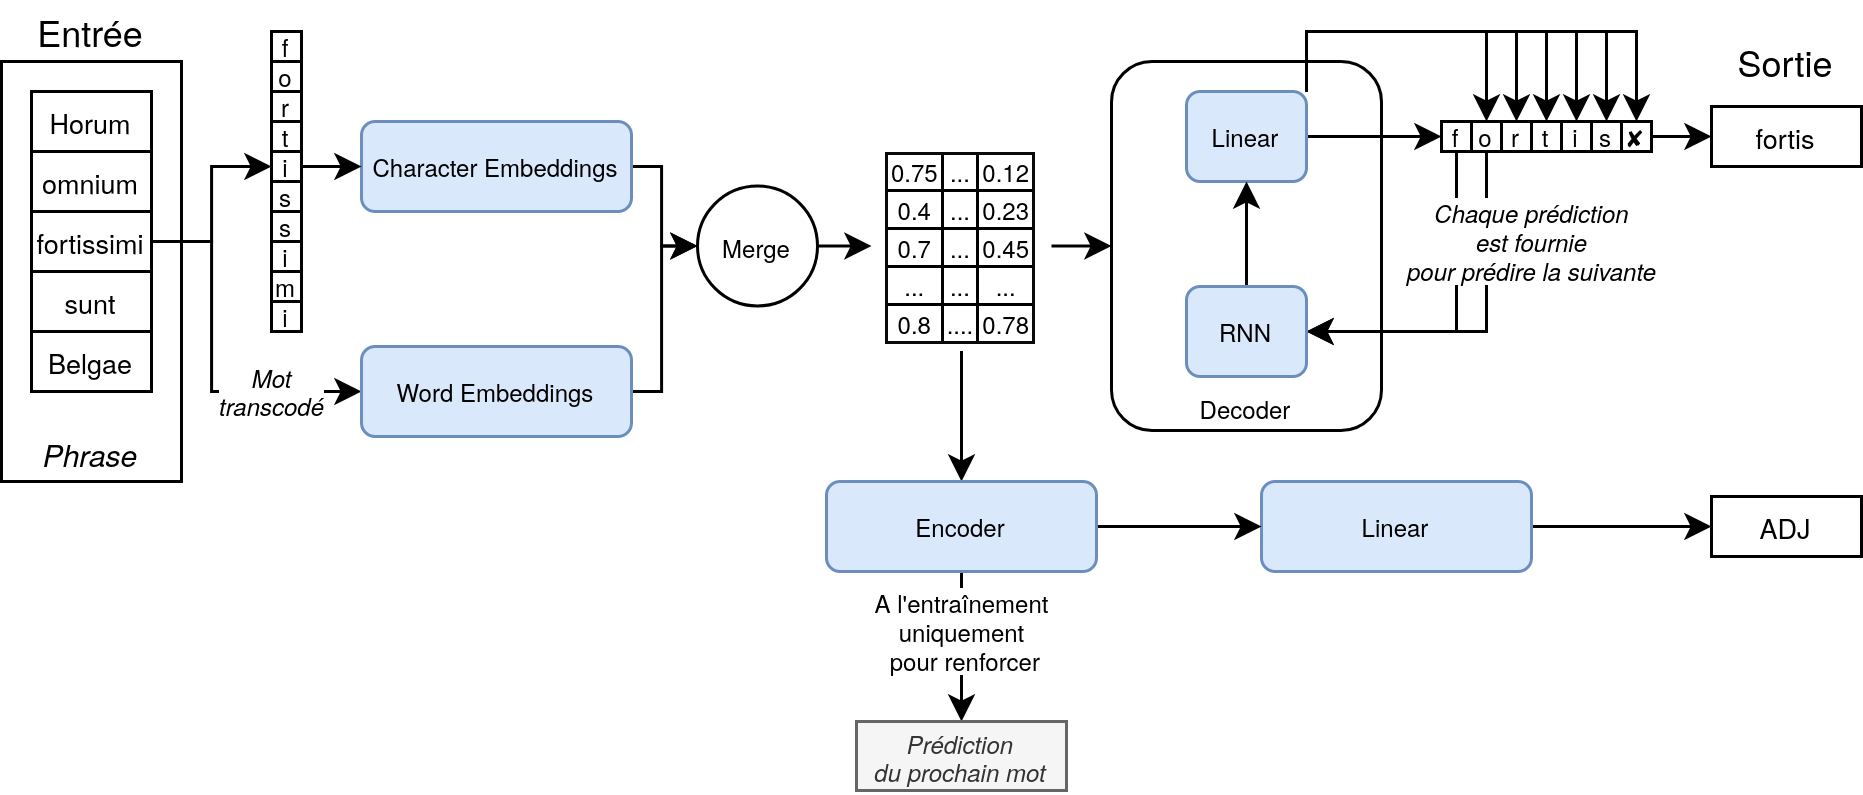
\includegraphics[width=.8\linewidth]{nlp-for-ch/images/Pie.png}
\end{frame}

\begin{frame}{PaPie}
    \begin{columns}
        \begin{column}{0.6\textwidth}
            \begin{itemize}
                \item Addition of optimizations for inference,
                \item Addition of random noise (e.g., capitalizing a word or a sentence),
                \item Optimizer and LR ({\small\url{https://github.com/lessw2020/Ranger-Deep-Learning-Optimizer}}),
                \item Other targets in score for dev.
            \end{itemize}
        \end{column}
        \begin{column}{0.4\textwidth}
        \vspace{1em}
            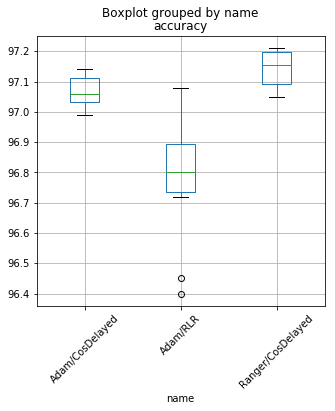
\includegraphics[width=\linewidth]{nlp-for-ch/images/boxplot_accuracy_ranger.png}
        \end{column}
    \end{columns}
\end{frame}

\section{Annotating Latin Texts}

\subsection{Datasets and Situation}

\begin{frame}{Quick Reminder of the Latin Morphological System}

\begin{itemize}
    \item 6 cases (7 including the locative for certain words)
    \item 2 numbers (singular, plural)
    \item 3 genders (masculine, neuter, feminine)
    \item 3 persons (1st, 2nd, 3rd) (similar to French)
    \item 7 verbal moods (Indicative, Imperative, Subjunctive, Infinitive, Participle, Adjective, Gerund, Supine)
    \item 6 tenses (present, imperfect, perfect, pluperfect, future, future perfect)
    \item 4 "voices" (Active, Passive, Deponent, Semi-deponent)
    \item 3 degrees (Positive, Comparative, Superlative)
\end{itemize}

+ absence of marking
    
\end{frame}

\begin{frame}{Overview of Classical and Late Corpora}

\begin{table}[h]
\centering
\resizebox{\textwidth}{!}{%
\begin{tabular}{l|rrrrrr}
\toprule
        & Tokens             & Punctuation & Number     & Number  & Lemmas & Reference \\ 
        &                    & Included    & of Authors & of Texts & Unique & \\   \midrule
PROIEL  & 225~064            & No                  & 5                & 6  & 7~246              & Lewis\footnotemark\\
Perseus & 79~670             & Yes                 & 12               & 12 & 6~017              & Lewis \\
Harrington & 120~029             & Yes                 & 9               & 12 &  7~675             & Lewis\\
LASLA   & \textbf{1~630~825} & No                  & \textbf{18}                 &  \textbf{100+}     & 25~135          & Forcellini \\ \bottomrule
\end{tabular}%
}
\caption{Summary of information on the four available corpora. There are 137 works in the LASLA corpus, but some are unusual divisions, so we prefer to indicate 100+ here.}
\end{table}

\pause

\vspace{-.5em}

Problem, they differ in:
\begin{enumerate}
    \item \textbf{POS} and morphological \textbf{reference frameworks}
    \item \textbf{Lexicalizations} taken into account, even when the same lemma reference framework is used.
\end{enumerate}

\end{frame}

\begin{frame}{After the 6th Century}

Other late and medieval corpora exist, particularly through \textit{Universal Dependencies}: 

\begin{itemize}
    \item UD-LLCT (Late Latin Charter Treebank)
    \item UD-Universal Dante
    \item UD-ITTB (Index Thomisticus Treebank)
    \item PaLaFra (\url{https://www.palafra.org})
\end{itemize}

but they present the same issues regarding lemmas or annotation practices.

LiLa (Linking Latin) as a knowledge base project connecting reference frameworks (but it does not resolve all problems): \url{https://lila-erc.eu/}.
    
\end{frame}

\begin{frame}{Temporal Representativeness of the Corpus}

\begin{figure}
    \centering
    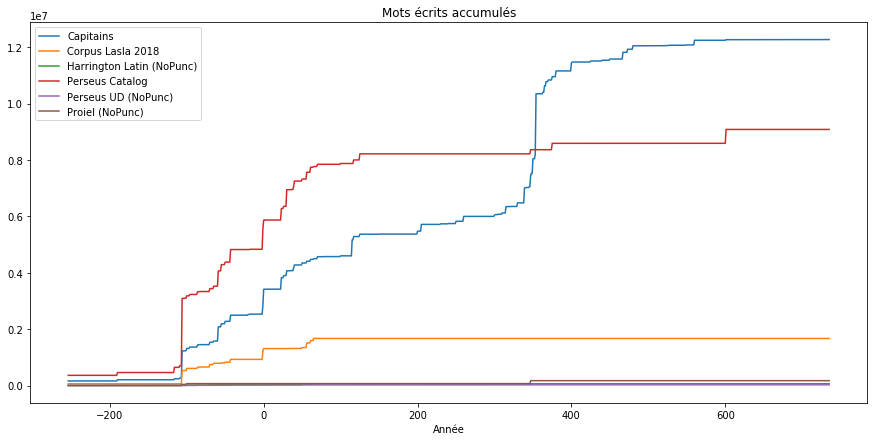
\includegraphics[width=.8\linewidth]{nlp-for-ch/images/lemmatisation_tokens_per_year.png}
    \caption{Accumulated words (Year of the author's birth)}
\end{figure}

\end{frame}

\begin{frame}{Problems of a Grammarian Corpus}
    \begin{columns}
        \begin{column}{.4\linewidth}
            \resizebox{\linewidth}{!}{%}
                \begin{tabular}{lll}
                    \toprule
                    Form & Mood & Tense \\ \midrule
                    amatus (sum) & Indicative & Perfect \\
                    amatus (eram) & Indicative & Pluperfect \\
                    amatus (ero) & Indicative & Future perfect \\
                    amatus (sim) & Subjunctive & Perfect \\
                    amatus (essem) & Subjunctive & Pluperfect \\
                    amatus (esse) & Infinitive & Perfect \\
                    amatum (iri) & Infinitive & Future \\ \bottomrule
                \end{tabular}
            }
            {\tiny Possible annotations for the form \textit{amatus} in LASLA, excluding participles.}
        \end{column}
        \begin{column}{.6\linewidth}
            Participle that carries the tense of the auxiliary in ellipsis.
            
            Other issues: debatable lemma forms (\textsc{paedico} $\rightarrow$ \textsc{pedico}), disambiguation sometimes linked to the \textbf{homography of canonical forms} but with \textbf{different morphology}, different \textbf{gender} (vallus1 / vallus2), or different \textbf{grammatical functions} (qui1, qui2, qui3, etc.) but sometimes also \textbf{semantic}.
        \end{column}
    \end{columns}
\end{frame}

\begin{frame}{Two New Corpora}

    \begin{itemize}
        \item \textbf{Sampling} \textit{From the 2nd century to Thomas More, a gold Latin corpus lemmatized and morphosyntactically annotated}, A. Glaise and T. Clérice, \texttt{[doi]10.5281/zenodo.6383162}. 57,000 tokens, 40 texts (usually 500 to 600 tokens), mainly 2 CE - 10 CE then 20,000 tokens from Jacques de Voragine and Thomas More.
        \item \textbf{Domain} \textit{Lemmatization and morphosyntactic analysis of the Priapea}, T. Clérice, \url{https://github.com/lascivaroma/priapea-lemmatization}.
    \end{itemize}

\end{frame}

\subsection{Training and Evaluating Models}

\begin{frame}{Model results}
    \vspace{1em}
    \begin{table}[ht]
        \resizebox{.8\linewidth}{!}{%}
        \begin{tabular}{l|rrr}
        \toprule
                         & \multicolumn{3}{l}{Accuracy}                           \\
                         & Known Forms & Unknown Forms &  Applicable Forms \\ \midrule
        Lemma            & 97.41          & 92.92            &                    \\
        POS              & 96.49          & 92.45            &                    \\
        Gender           & 96.28          & 91.49            &   89.98            \\
        Number           & 97.02          & 93.85            &   96.44            \\
        Case             & 92.34          & 87.37            &   87.84            \\
        Degree           & 98.07          & 93.96            &   93.37            \\
        Mood Tense Voice & 98.35          & 90.80            &   94.44            \\
        Person           & 99.71          & 98.15            &   98.49            \\ \midrule
        Aggregate Tasks  & 85.86          & 76.68            &                    \\ \bottomrule 
        \end{tabular}
        }
    \end{table}

\end{frame}

\begin{frame}{Training and Corpus Size (1)}

    \begin{center}
        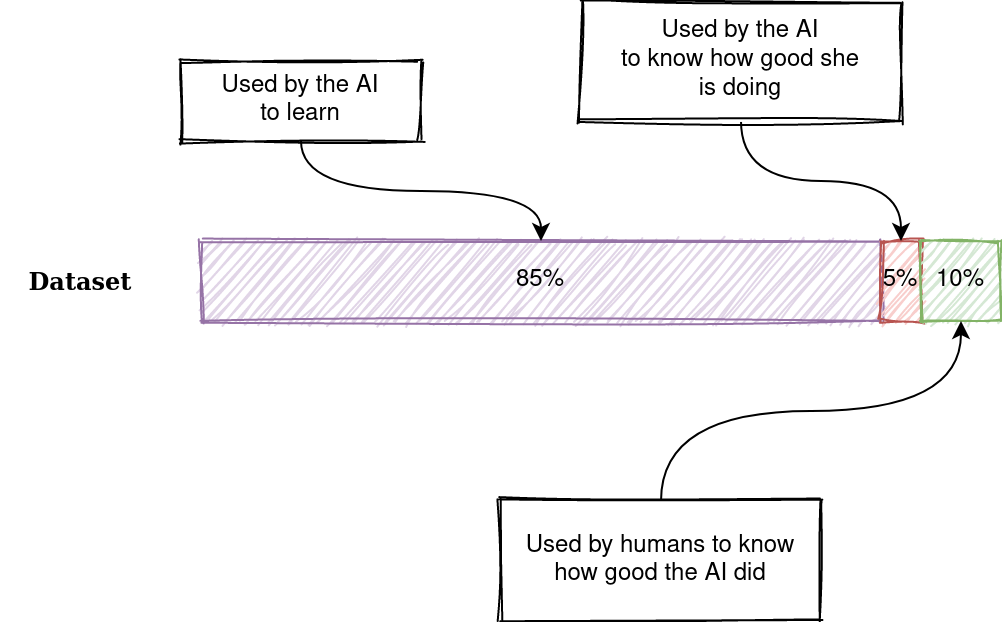
\includegraphics[width=\linewidth,height=0.8\textheight,keepaspectratio]{nlp-for-ch/images/lemma-dataset.png}
    \end{center}

\end{frame}

\begin{frame}{Training and Corpus Size (2)}

    \begin{table}[]
        \centering
        \begin{tabular}{lr|rrrr}
        \toprule
         RNN &  \% Corpus &  Lemma &  $\Delta$(Lemma) &  $\theta$ Lemma &  $\Delta$($\theta$ Lemma) \\
        \midrule
           1 &     1.0 &  0.741  &     0.000 &    0.725 &       0.000 \\
           1 &     5.0 &  0.889  &     0.149 &    0.858 &       0.133 \\
           2 &     7.5 &  0.921  &     0.031 &    0.855 &      -0.002 \\
           2 &     10.0 &  0.936 &     0.015 &    0.894 &       0.039 \\
           2 &     20.0 &  0.949 &     0.013 &    0.882 &      -0.012 \\
           2 &     40.0 &  0.968 &     0.019 &    0.922 &       0.041 \\
           2 &     60.0 &  0.970 &     0.002 &    0.924 &       0.002 \\
           2 &     80.0 &  0.975 &     0.005 &    0.910 &      -0.014 \\
        \bottomrule
        \end{tabular}
    \end{table}
    
    
    \small The gain measurements between two stages, denoted by $\Delta$, correspond to the difference with the previous model, so read as “The model with 80\% of the corpus performs 0.46 points better than the model with 60\% of the corpus.” We also add a measure on an out-of-domain corpus, that of late Latin, referred to in the columns by a $\theta$.

\end{frame}

\begin{frame}{Error Analysis on out of domain}
    \only<1>{
        \centering
        \fullcite{clerice_2022_6383163}
        \begin{tabular}{l|rrrrrrr}
        \toprule
        Century & 2 & 3 & 5 & 6 & 7 & 7 & 9 \\ \midrule
        Authors & 1 & 3 & 5 & 4 & 2 & 1 & 1 \\
        Texts   & 2 & 3 & 6 & 4 & 2 & 1 & 1 \\ \bottomrule
        \end{tabular}
    }
    \only<2>{
        \centering
        \begin{tabular}{l|rr|rr}
            \toprule
                 Catégorie &  \multicolumn{2}{c}{\textit{Accuracy}} & \multicolumn{2}{c}{\textit{Accuracy} quand applicable} \\
            \midrule    
                        {} &  Priapées &    Tardif                  & Priapées &    Tardif                                   \\
            \midrule
                     lemma &     94,2 &    94,5                   &   N/A    &    N/A                                      \\
                       Deg &     96,8 &    97,5                   &   90,3   &    91,5                                     \\
                      Numb &     94,7 &    96,5                   &   94,1   &    96,4                                     \\
                    Person &     99,0 &    99,7                   &   96,0   &    99,1                                     \\
        Mood\_Tense\_Voice &     96,1 &    97,7                   &   87,0   &    92,3                                     \\
                      Case &     89,4 &    92,9                   &   84,1   &    88,0                                     \\
                      Gend &     91,7 &    92,8                   &   77,8   &    79,2                                     \\
                       pos &     95,0 &    67,6                   &   N/A    &    N/A                                      \\
            \bottomrule
        \end{tabular}
    }
\end{frame}

\begin{frame}{Error Analysis on out of domain (2)}
    \begin{figure}[ht]
        \centering
        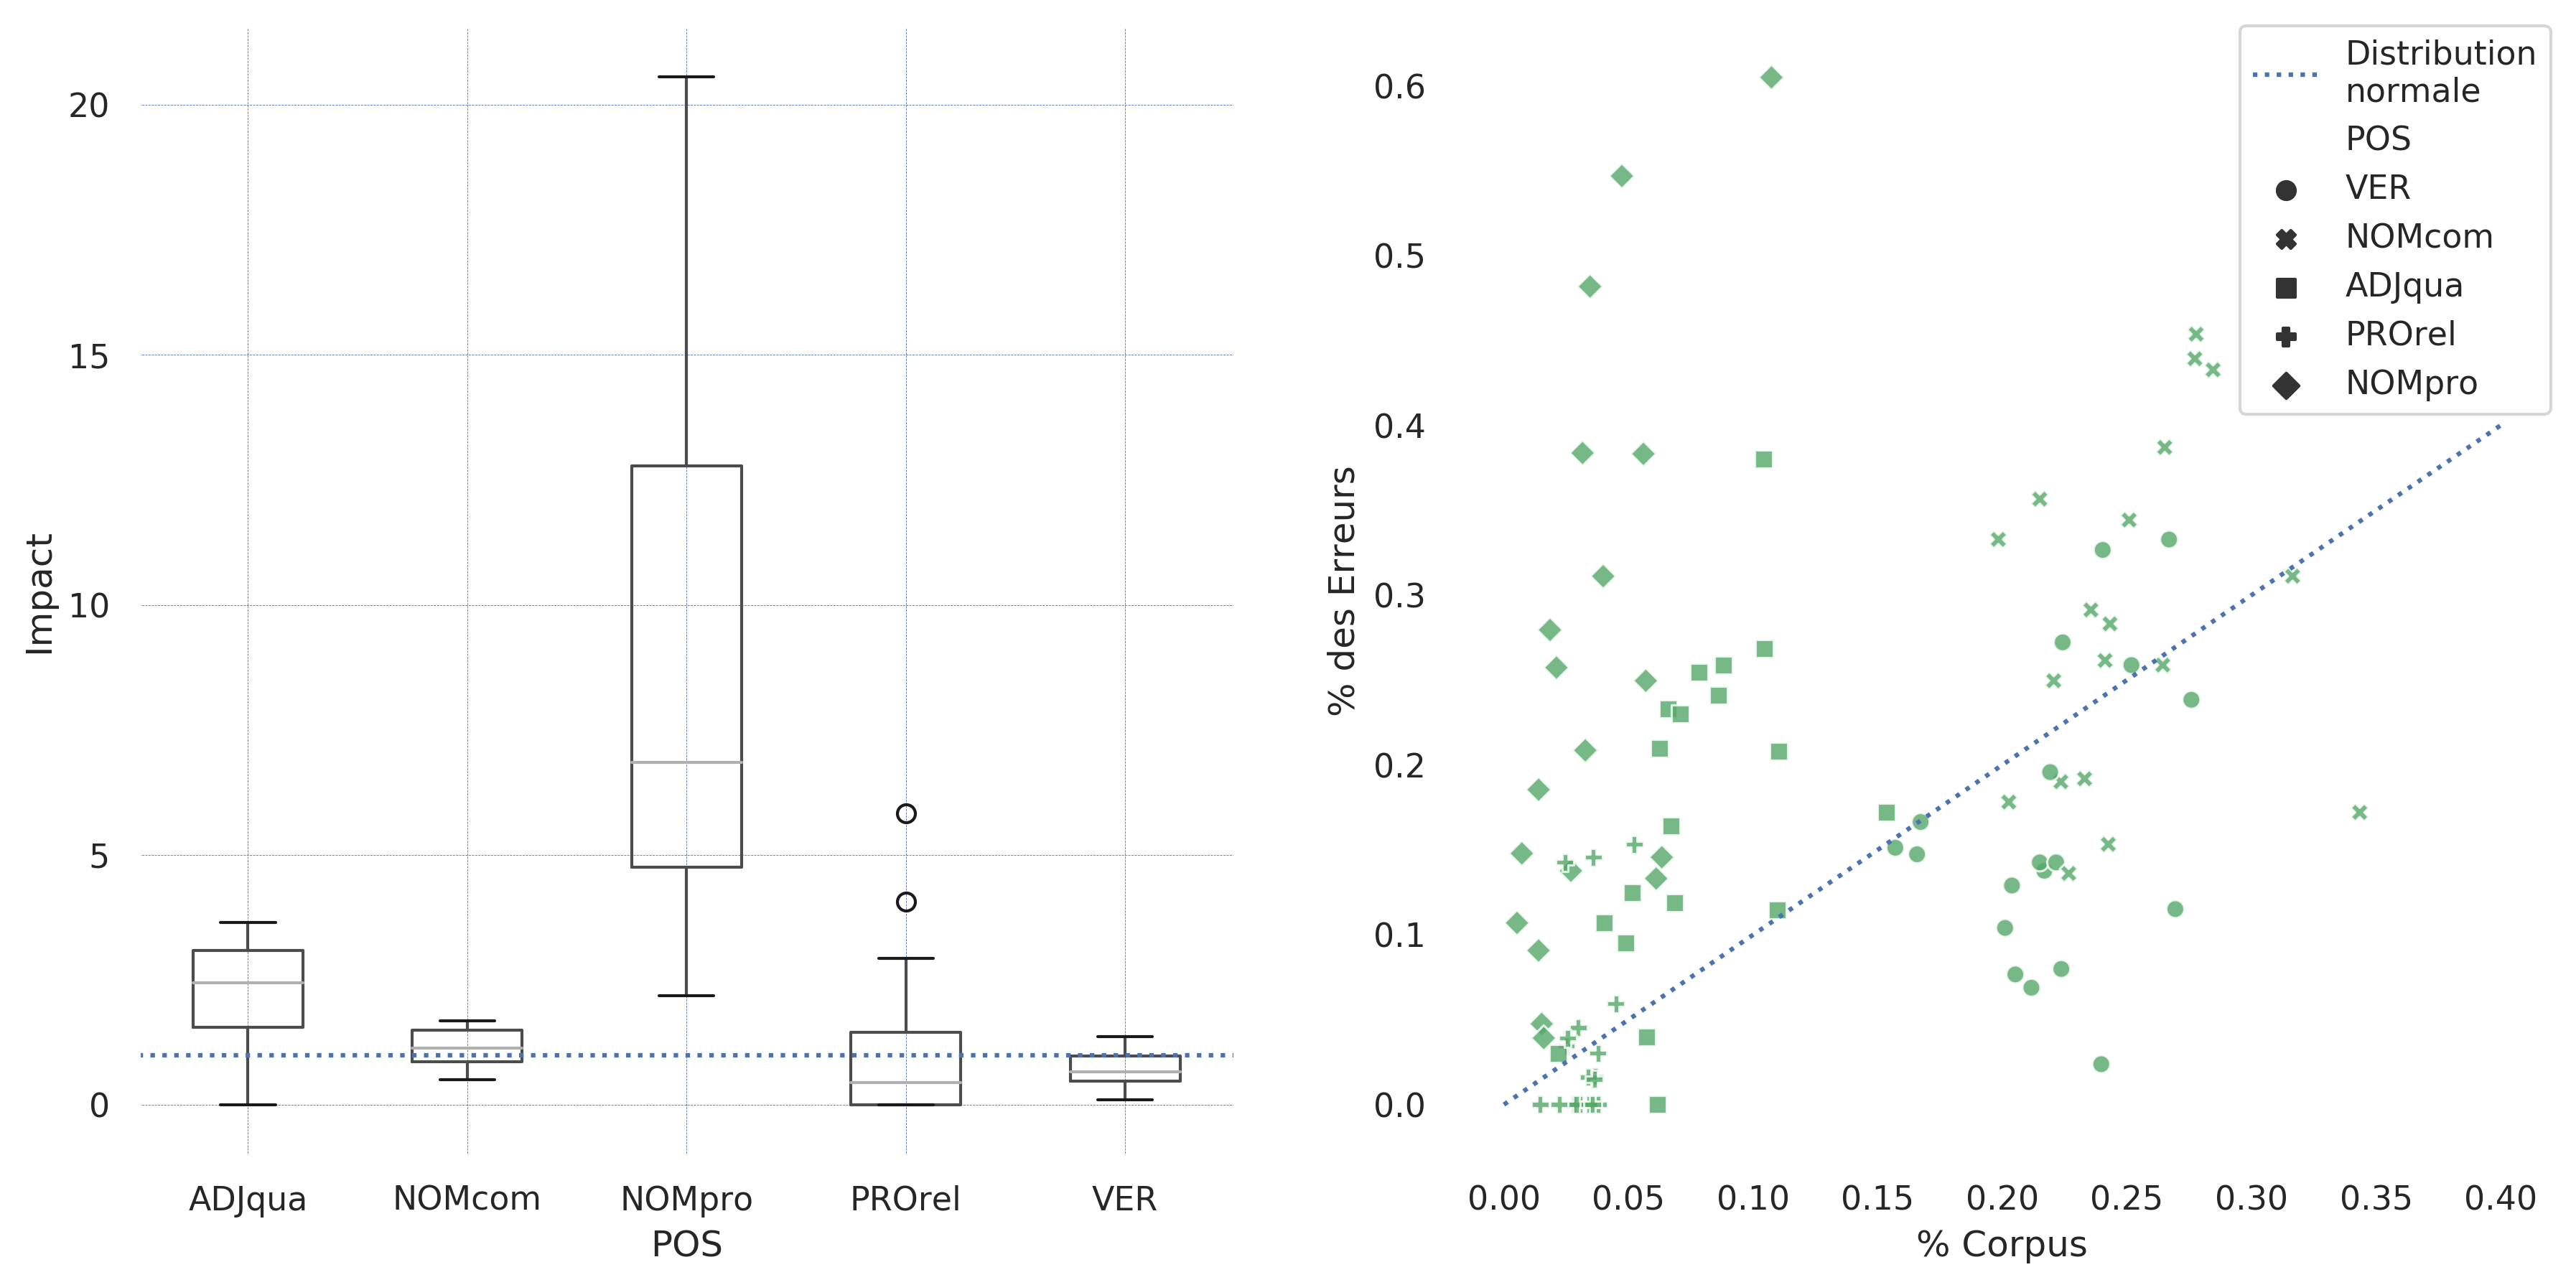
\includegraphics[width=.85\linewidth]{images/LatinTardifPosErrorBoxPlot.png}
        \caption{Proportion of errors per category on the "Late Antiquity" Corpora.}
    \end{figure}
\end{frame}

\begin{frame}{Error Analysis on out of domain (3)}
    \textbf{Main Error Categories in Proper Nouns}

    \begin{itemize}
        \item \textbf{Unrecognized Proper Noun:} Lemma mistaken for a common noun 
        (e.g., \textsc{terra} vs. \textsc{Terra}, *\textsc{uenus} vs. \textsc{Uenus}).
        \item \textbf{Singular/Plural Confusion:} Common in ethnonyms (\textsc{Graecus} vs. \textsc{Graeci}).
        \item \textbf{Greek/Hebrew Origin:} Terms like \textsc{Christus}, \textsc{Israel}, which rarely appear in training data.
        \item \textbf{Latin Graphical Variation:} Pairs like \textit{Bethleem}/\textit{Bethlehem}, \textit{Hadrianus}/\textit{Adrianus}.
    \end{itemize}
    \pause
    \textbf{Additional Error Types}
    
    \begin{itemize}
        \item \textbf{Root Selection:} Choosing incorrect root (\textit{debeo} vs. \textit{debitum}).
        \item \textbf{Common Noun as Proper Noun:} Misleading capitalization.
        \item \textbf{Reconstruction Error:} Confusing noun/adjective 
        (\textit{prophetia}/\textit{prophetius}).
        \item \textbf{Spelling Issues:} "Reactionary" spelling errors (\textit{pedico} vs. \textit{paedico}).
    \end{itemize}
    
\end{frame}


\begin{frame}{The issue of highly curated data}

    \only<1>{
        \begin{figure}[ht]
            \textit{Bellum Gallicum}, {Caesar}
            \begin{description}
                \item[Source] Gallia omnis divisa in partes tres , quarum unam incolunt Belgae , aliam Aquitani tertiam , qui ipsorum lingua Celtae nostra Galli appellantur.
                \item[Raw] gallia omnis \textbf{dico} in pars tres \textbf{qvi} qvi vnvs incolo belgae \textbf{vnde} alivs aqvitani tertivs \textbf{vi} qvi ipse lingva celtae noster galli appello \textbf{nonvs}.
                \item[Norm.] gallia omnis divido in pars tres , qvi vnvs incolo belgae , alivs aqvitani tertivs , qvi ipse lingva celtae noster galli appello .
            \end{description}
            \caption{Example of noise caused in lemmatization when no preprocessing is performed. In bold are the errors introduced by the lemmatization: we notice that aside from the completely incorrect lemmatization of the punctuation marks, divisa is also poorly analyzed, likely due to the noise from punctuation and the letter "v."}
            \label{quote:lemmatisation:gallia-errors}
        \end{figure}
    }
    
    \only<2>{
        \begin{table}[ht]
            \centering
            \resizebox{\linewidth}{!}{%
            \begin{tabular}{l|rrrr}
            \toprule
                                                      & A                 & B                 & C              & D              \\ \midrule
            Ramist Letters normalization              & No                & Yes               & No             & Yes            \\
            Removal of punctuation                    & No                & No                & No             & Yes            \\
            Tokenisation Phrase                       & Sentences Markers & Sentences Markers & 35 Words       & 35 Words       \\ \midrule
            lemma              & \textbf{-1,51} & -0,22          & \textbf{-1,62} & -0,23 \\
            Deg                & -0,30          & -0,16          & -0,26          & -0,06 \\
            Numb               & -0,41          & -0,31          & \textbf{-0,56}          & -0,12 \\
            Person             & -0,05          & 0,00           & -0,06          & -0,03 \\
            Mood\_Tense\_Voice & -0,11          & -0,02          & -0,12          & -0,04 \\
            Case               & \textbf{-0,76} & \textbf{-0,66} & \textbf{-1,41} & \textbf{-0,32} \\
            Gend               & -0,28          & -0,13          & -0,23          & -0,11 \\
            pos                & \textbf{-0,57} & -0,33          & \textbf{-0,66} & -0,18 \\ \bottomrule
            \end{tabular}}
            \caption{Impact of normalization on accurasy, in percentage points.}
            \label{tab:lemmatisation:normalisation}
        \end{table}
    }
\end{frame}

\section{Infrastructure}

\begin{frame}{Applications}

\begin{center}
    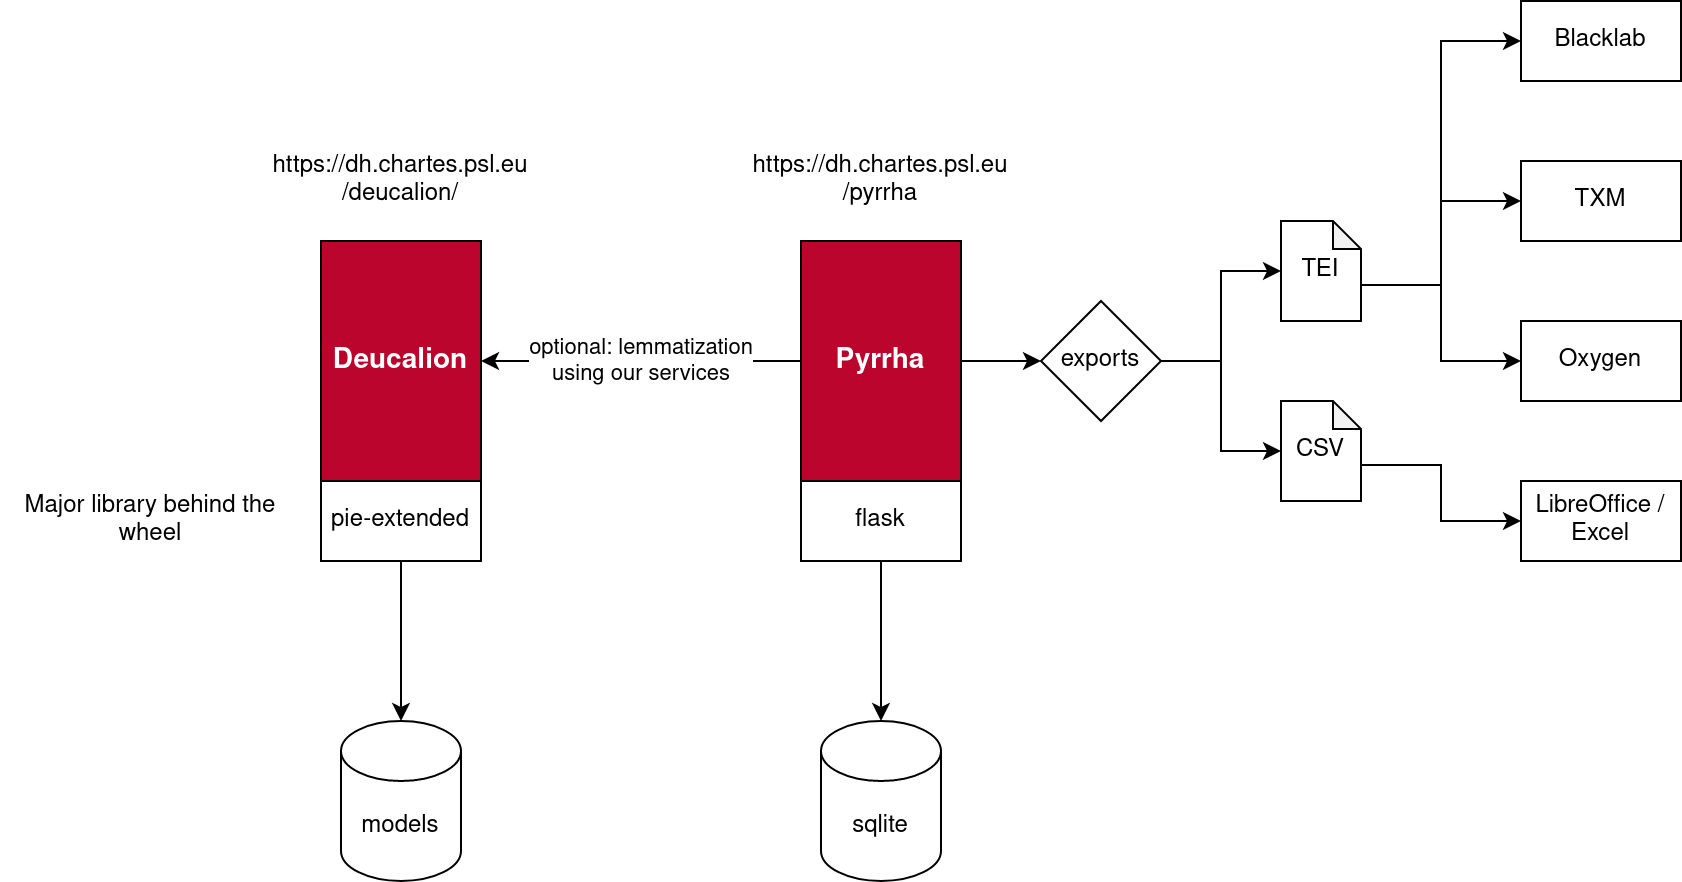
\includegraphics[width=\linewidth,height=0.8\textheight,keepaspectratio]{nlp-for-ch/images/infra-applis.png}
\end{center}
    
\end{frame}

\begin{frame}{Lemmatizers and Their Cycles}

\begin{center}
    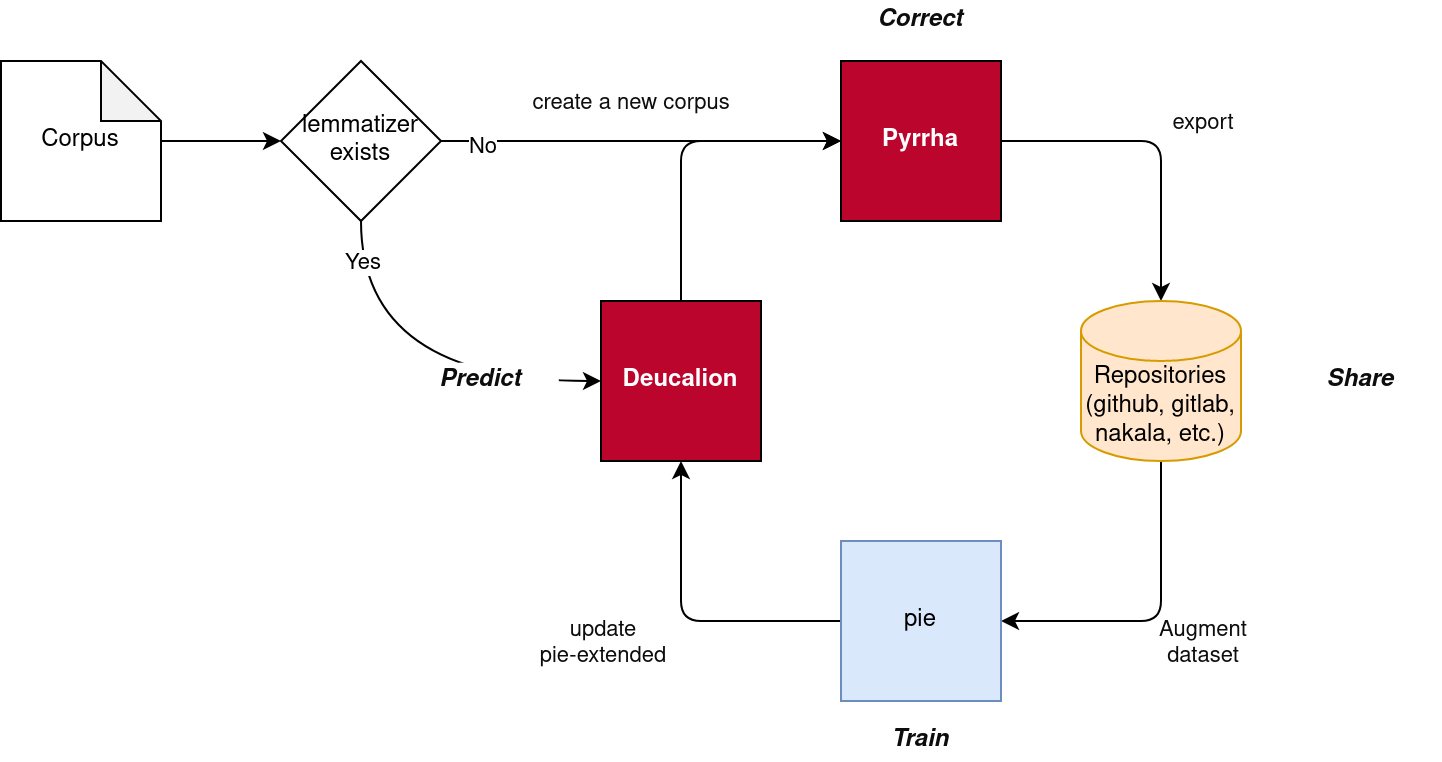
\includegraphics[width=\linewidth,height=0.8\textheight,keepaspectratio]{nlp-for-ch/images/infra-cycle.png}
\end{center}

\end{frame}

\end{document}
